\chapter{Analiza wymagań}
\label{cha:analizaWymagan}

%---------------------------------------------------------------------------

\section{Koncepcja cyfrowego zarzadzania tozsamosciami(IdM)}
\label{sec:konceptcjaIdM}

Zarządzanie tożsamościami(Identity Management) jest podejściem do zagadnienia zapewnienia bezpieczeństwa dostępu do aplikacji w oparciu o dane identyfikujące użytkownika(Identity). Pojęcie danych identyfikujących może być zdefiniowane jako "informacje o jednostce pozwalające na identyfikację tej jednostki dla pewnej dziedziny zastosowań"\cite{Itu09}. W kontekście systemów zarządzania cyfrowymi tożsamościami dane identyfikujące mogą dotyczyć nie tylko osób ale również na przykład komponentów programowych\cite{Bertino11}. Zgodnie z rekomendacją Y.2720 w skład danych identyfikujących wchodzą identyfikator jednostki, dane uwierzytelniające jednostkę oraz atrybuty opisujące jednostkę\cite{Itu09}.

Elisa Bertino i Kenji Takahashi w książce "Identity Management" definiują cele zarządzania tożsamościami jako "utrzymanie integralności danych identyfikujących w trakcie ich użytkowania w celu udostępniania tych danych i powiązanych z nimi informacji w sposób bezpieczny i chroniący prywatność użytkowników"\cite{Bertino11}.
 
\subsection{Role w koncepcji systemów zarządzania tożsamościami}

Systemy zarządzania tożsamościami charakteryzują się rozdzieleniem odpowiedzialności związanych z dostarczaniem funkcjonalności oraz zadań związanych z zapewnieniem bezpieczeństwa dostępu do aplikacji. Usługi uwierzytelniania i autoryzacji oraz funkcjonalności systemów dostarczane są dla jednostek - składowych systemu zarządzania tożsamościami - zazwyczaj użytkowników.
Dane identyfikacyjne jednostek są gromadzone i wykorzystywane w trakcie korzystania z aplikacji. Dane osobowe mogą obejmować informacje związane z dokumentami tożsamości(numery dowodu osobistego, paszportu), dane bankowe, biometryczne oraz informacje związane z przebiegiem interakcji jednostki z systemem. Dane identyfikacyjne jednostek powinny być przetwarzane i gromadzone w sposób zapewniający  ochronę przed niewłaściwym użyciem. Nadużycia danych osobowych jednostek mogą prowadzić do istotnych strat użytkowników aplikacji.
Elementem przeprowadzającym weryfikację tożsamości jednostek jest usługa "Identity Provider"(IdP). Usługa ta odpowiedzialna jest za przyporządkowywanie jednostkom atrybutów opisujących tożsamość, tworzenie powiązań pomiędzy różnymi atrybutami jednostki oraz tworzenie asercji zawierających informacje o atrybutach jednostek. 

Usługa 'Identity Provider' może współpracować z innymi usługami tego typu dołączając do danych uwierzytelniających informacje udostępniane przez inne zaufane usługi IdP. Wykorzystanie danych uwierzytelniających dostarczanych przez inne usługi uwierzytelniające wymaga wprowadzenia procesu zapewnienia wiarygodności otrzymywanych danych. Proces ten może opierać się na przypisywaniu miary wiarygodności do atrybutów uwierzytelniających. Wyznaczenie wartości tej miary może być na przykład oparte o ocenę stopnia zaawansowania mechanizmów weryfikacji danych uwierzytelniających wykorzystywanych przez usługę dostarczająca dany atrybut tożsamości.

Dostawcy usług wykorzystujący infrastrukturę systemów zarządzania tożsamościami przed zezwoleniem na dostęp do swoich zasobów zlecają usługom typu IdP przeprowadzenie procesu uwierzytelniania klienta na podstawie otrzymanych danych uwierzytelniających. Dostawcy usług powinni mieć możliwość deklaracji poziomu skuteczności zabezpieczeń wykorzystywanych w procesie autoryzacji dostępu do określonych zasobów. Poziom ten może być różny w zależności od rodzaju zasobu.

Przedstawiona w książce "Identity Management Concepts, Technologies, and Systems" terminologia wprowadza również pojęcie jednostki nadzorującej\cite{Bertino11}. Jest to najczęściej instytucja upoważniona prawnie do nadzoru nad procesami przetwarzania i przechowania danych osobowych lub wglądu  w informacje o charakterze poufnym.

\subsection{Relacje miedzy rolami w systemach zarządzania tożsamościami}

	\begin{figure}[h]
		\centering
		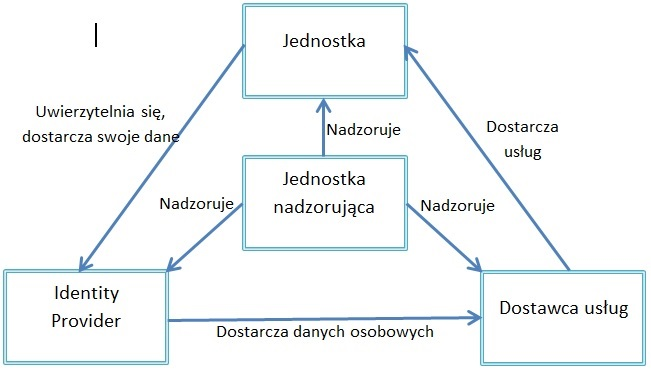
\includegraphics[width=15cm]{img/idmRelations.jpg}
		\caption{Relacje miedzy rolami w systemach zarządzania tożsamościami}
		\label{Relacje miedzy rolami w systemach zarządzania tożsamościami}
	\end{figure}

	Często stosowanym modelem jest infrastruktura złożona z jednej usługi typu "Identity Provider" oraz wielu usług funkcjonalnych opierających na niej swoje mechanizmy zabezpieczeń. Dzięki takiemu rozwiązaniu dostawcy usług mogą skoncentrować się na tworzeniu funkcjonalności stanowiących istotę aplikacji - odpowiedzialności związane z zapewnieniem bezpieczeństwa dostępu delegowane są do usługi IdP. Specjalizowana usługa uwierzytelniania może dostarczać bardziej zaawansowanych zabezpieczeń. Dzięki realizacji tego modelu użytkownicy nie muszą zarządzać wieloma danymi uwierzytelniającymi dla różnych usług - dostęp do wielu serwisów gwarantowany jest przy użyciu tych samych danych. Wprowadza to jednak zagrożenia związane z centralizacja dostępu do różnych usług.

\subsection{Federated Identity Management}

Najczęściej użytkownicy korzystają nie z jednej usługi lecz z szerokiej gamy różnych usług. Każda z usług korzysta z własnych danych uwierzytelniających. Podejście "Federated Identity Management" umożliwia tworzenie powiązań pomiędzy tożsamościami użytkownika w ramach różnych usług dzięki czemu dane uwierzytelniające każdej z sfederowanych usług mogą być wykorzystane w procesie uwierzytelniania dowolnej z usług.

\subsection{Cykl życia tożsamości}

Jednym z głównych zadań systemów zarządzania tożsamościami jest kontrola nad cyklem życia tożsamości. Autorzy książki "Identity Management: Concepts, Technologies and Systems" opisują 4 etapy cyklu życiu tożsamości: tworzenie, użytkowanie, aktualizacja oraz wycofanie z użycia\cite{Bertino11}.

Proces tworzenia cyfrowej tożsamości składa się z kilku kroków. Pierwszym z nich może być weryfikacja przedstawionych atrybutów tożsamości, wymagająca udowodnia przez jednostkę prawdziwości wprowadzanych danych. Następnie tworzone są dane uwierzytelniające. Ostatnim krokiem jest utworzenie tożsamości na podstawie otrzymanych danych oraz nadanie jednostce identyfikatora.

Utworzona tożsamość może być wykorzystywana w różnych celach, np. zapewnienia wiarygodnej komunikacji lub w procesie jednokrotnego uwierzytelniania(ang. Single Sign-On).

Systemy zarządzania tożsamościami powinny obsługiwać zmiany atrybutów tożsamości. Powinny aktualizować informacje o danych jednostek po zmianach wysyłając powiadomienia do usług przechowujących te dane, np. "Identity Provider". Identyfikatory jednostek nie powinny podlegać zmianom. Systemy IdM muszą również usuwać tożsamości jeśli nie są już aktualne.

\section{Jednokrotne uwierzytelnianie}

Książka "Identity Management: Concepts, Technologies and Systems" definiuje jednokrotne uwierzytelnianie(ang. Single Sign-On) jako proces uwierzytelniania, w którym jednostka może wykorzystać wynik pojedynczego uwierzytelniania dla uzyskania dostępu do wielu niezależnych usług z ochroną dostępu\cite{Bertino11}. 

Podstawą funkcjonowania mechanizmów jednokrotnego uwierzytelniania jest nawiązanie relacji zaufania pomiędzy dostawcami usług oraz serwisami typu "Identity Provider". Po uwierzytelnieniu użytkownika w ramach jednej z usług objętych mechanizmem SSO dostęp do innej nie wymaga uwierzytelniania - dane uwierzytelniające są mapowane na dane niezbędne do uwierzytelnienia względem innej usługi oraz generowane są informacje pozwalające na uzyskanie dostępu do serwisu. Usługi korzystające z mechanizmu jednokrotnego uwierzytelniania powinny otrzymywać informacje kontekstowe o przebiegu procesu uwierzytelniania takie jak: wykorzystywane metody uwierzytelniania oraz sposób ochrony danych uwierzytelniających. Informacje te pozwalają na ocenę stopnia wiarygodności przeprowadzonego procesu uwierzytelniania.

\subsubsection{Architektura systemów jednokrotnego uwierzytelniania}

Implementacja mechanizmu jednokrotnego uwierzytelniania może opierać się o różne architektury. Autorzy książki "Identity Management: Concepts, Technologies and Systems"\cite{Bertino11} wymieniają następujące typy architektur systemów jednokrotnego uwierzytelniania:

\begin{itemize}
  \item Architektura oparta o brokery - architektura składająca się z punktu centralnego(serwera) oraz jednostek przez niego uwierzytelnianych. Serwer przydziela użytkownikom tokeny uwierzytelniające, dzięki którym możliwy jest dostęp do aplikacji. Przykładem architektury tego typu jest protokół Kerberos. 
  \item Architektura oparta o agenty - architektura, w której w dostępie do każdej aplikacji pośredniczy agent uwierzytelniania. Jego rolą jest translacja pomiędzy metodą uwierzytelniania zastosowaną przez klienta a mechanizmami obsługiwanymi przez aplikację.
  \item "Reverse proxy-based architecture" - architektura wprowadzająca usługę proxy pośredniczącą w dostępie do wszystkich aplikacji objętych procedurą SSO. Moduł proxy dokonuje filtrowania przychodzących komunikatów - nieuwierzytelnione żądania zostają przekierowane, np. do serwera uwierzytelniającego.
\end{itemize}
  
Procedura jednokrotnego uwierzytelniania pozwala na wygodniejszy sposób korzystania z aplikacji - znosi konieczność wielokrotnego wprowadzania danych identyfikujących. Użytkownik nie musi też zapamiętywać wielu haseł dla różnych usług. Wiele prostych haseł może zostać zastąpionych jedną bardziej wiarygodną metodą uwierzytelniania(np. z wykorzystaniem bardziej skomplikowanego hasła). Wadą wprowadzenia procedury jednokrotnego uwierzytelniania jest jednak centralizacja punktu dostępu do różnych aplikacji - złamanie zabezpieczeń otworzy drogę do wielu usług użytkownika.

%---------------------------------------------------------------------------

\section{Service-Oriented Architecture}
\label{sec:soa}

Service-Oriented Architecture

%---------------------------------------------------------------------------

\section{Wymagania stawiane systemom Business-to-Business}
\label{sec:wymaganiaB2B}

Wymagania stawiane systemom Business-to-Business

%---------------------------------------------------------------------------

\section{Zakres wymagan tworzonego systemu}
\label{sec:zakresWymagan}

Zakres wymagan tworzonego systemu

